\documentclass[nosubsub]{maps}

%\documentclass[onecolumn]{maps} % for symmetric single-column layout

\usepackage{url}
\usepackage{graphicx}
\usepackage{eurosym} % for the euro symbol

\renewcommand{\notesname}{Footnotes}

% title- and author commands can be placed before or after
% \begin{document}.

\setcounter{page}{2}

\begin{document}

\title{\TeX{} on the Road}

\subtitle{An adventure with \TeX{} while traveling light}

\author[Piet van Oostrum]{Piet van Oostrum\\
  \texttt{piet@vanoostrum.org}\\
  \url{http://piet.vanoostrum.org}}

\maketitle

\begin{abstract}
This article describes the adventures that I had while working on a small \TeX{} project without my beloved laptop at hand. With only an iPad to do the work and without a local \TeX{} system installed on it, there were several challenges. I document them here so that others can enjoy the struggles I had and can benefit from the solutions when they encounter similar situations.
\end{abstract}

\begin{keywords}\TeX, traveling, iPad, Overleaf, git, distributed version management, Github
\end{keywords}

\section{The context}

In July 2018, my wife Cary and I were traveling in South America, to visit friends in Brazil and Bolivia, and additionally to have some vacation. We wanted to travel light, so I had decided not to take my MacBook with me, saving a little bit more than 2 kgs.\ of weight. We both had our iPhones and iPads (mine is an iPad mini), and we hoped that would do. They were mainly to be used for reading email, interactions on social media, searching for city and transport information, and the like.
\begin{figure}[b]
  \centering
  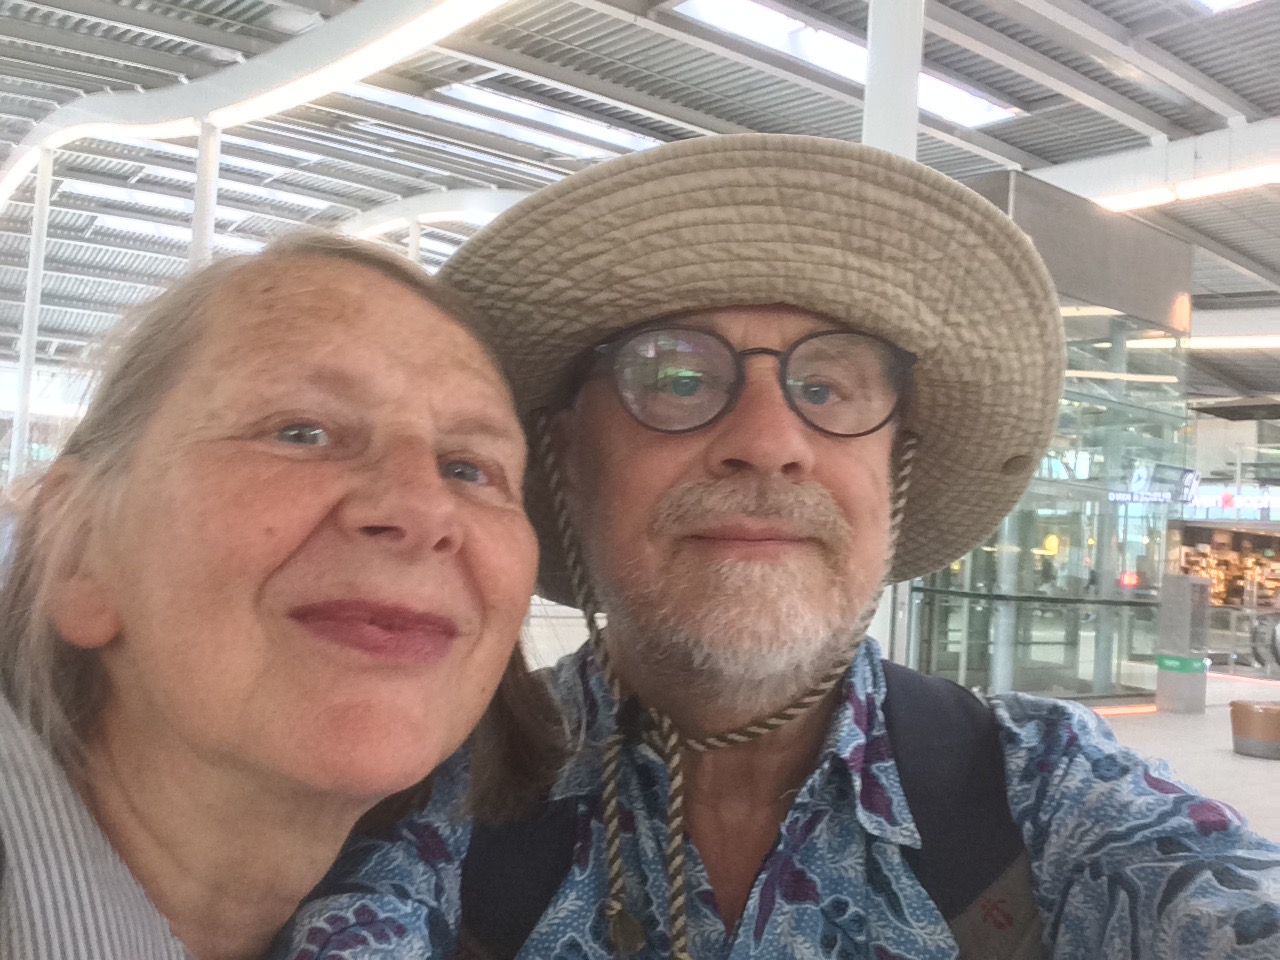
\includegraphics[width=0.9\columnwidth]{foto}
  \caption{On our way to Brazil}
\end{figure}

I did not expect to do any \TeX{} work, maybe some light programming, for which I had a Python system (Pythonista)\footnote{\url{http://omz-software.com/pythonista/}} on my iPad.

While we were traveling in Brazil, on our way to Bolivia, I got an email from a user of the \texttt{multirow} package about a possible bug. It came with a solution which was a very simple substitution, and back home on the laptop, it would have been a few minutes to make the change, check it in into the version control system, do some test, generate a new version of the documentation, and upload the new version to CTAN.

Because this person had already made a local change, and the problem was not urgent anyway, my first reaction was: I will correct it when I am back home, which, by the way, would be some 2 months later. However when we arrived in Bolivia, where we were staying a couple of weeks, the temptation to solve the problem right there became too large.

But what would have taken at most 10 minutes at home, became a major effort without having a computer with a \TeX{} system. In the end it took me more than two days of struggling, but with  victory in the end.

If I would have distributed the package just as a collection of \texttt{.sty} files (there are three included), with a separate documentation, the task would have been simple. I could have downloaded the package from CTAN, changed the \texttt{.sty} files with a text editor in my iPad, and uploaded them back to CTAN. It might have caused some frowning from the CTAN maintainers if the version number in the documentation would have been different from the one in the \texttt{.sty} files, but that would have been temporary anyway.

However, the package was distributed as a \texttt{.dtx} file, with a corresponding \texttt{.ins} file, and a separate PDF file containing the documentation which is generated from the \texttt{.dtx} file. The \texttt{.sty} files are also generated from the \texttt{.dtx} file with the aid of the \texttt{.ins} file. This is the standard setup for most CTAN packages. But this requires the \texttt{.dtx} and \texttt{.ins} files to be processed by \LaTeX{} (or \TeX{} in case of the \texttt{.ins} file). And I did not have a \LaTeX{} distribution on my iPad.

\begin{figure}
  \centering
  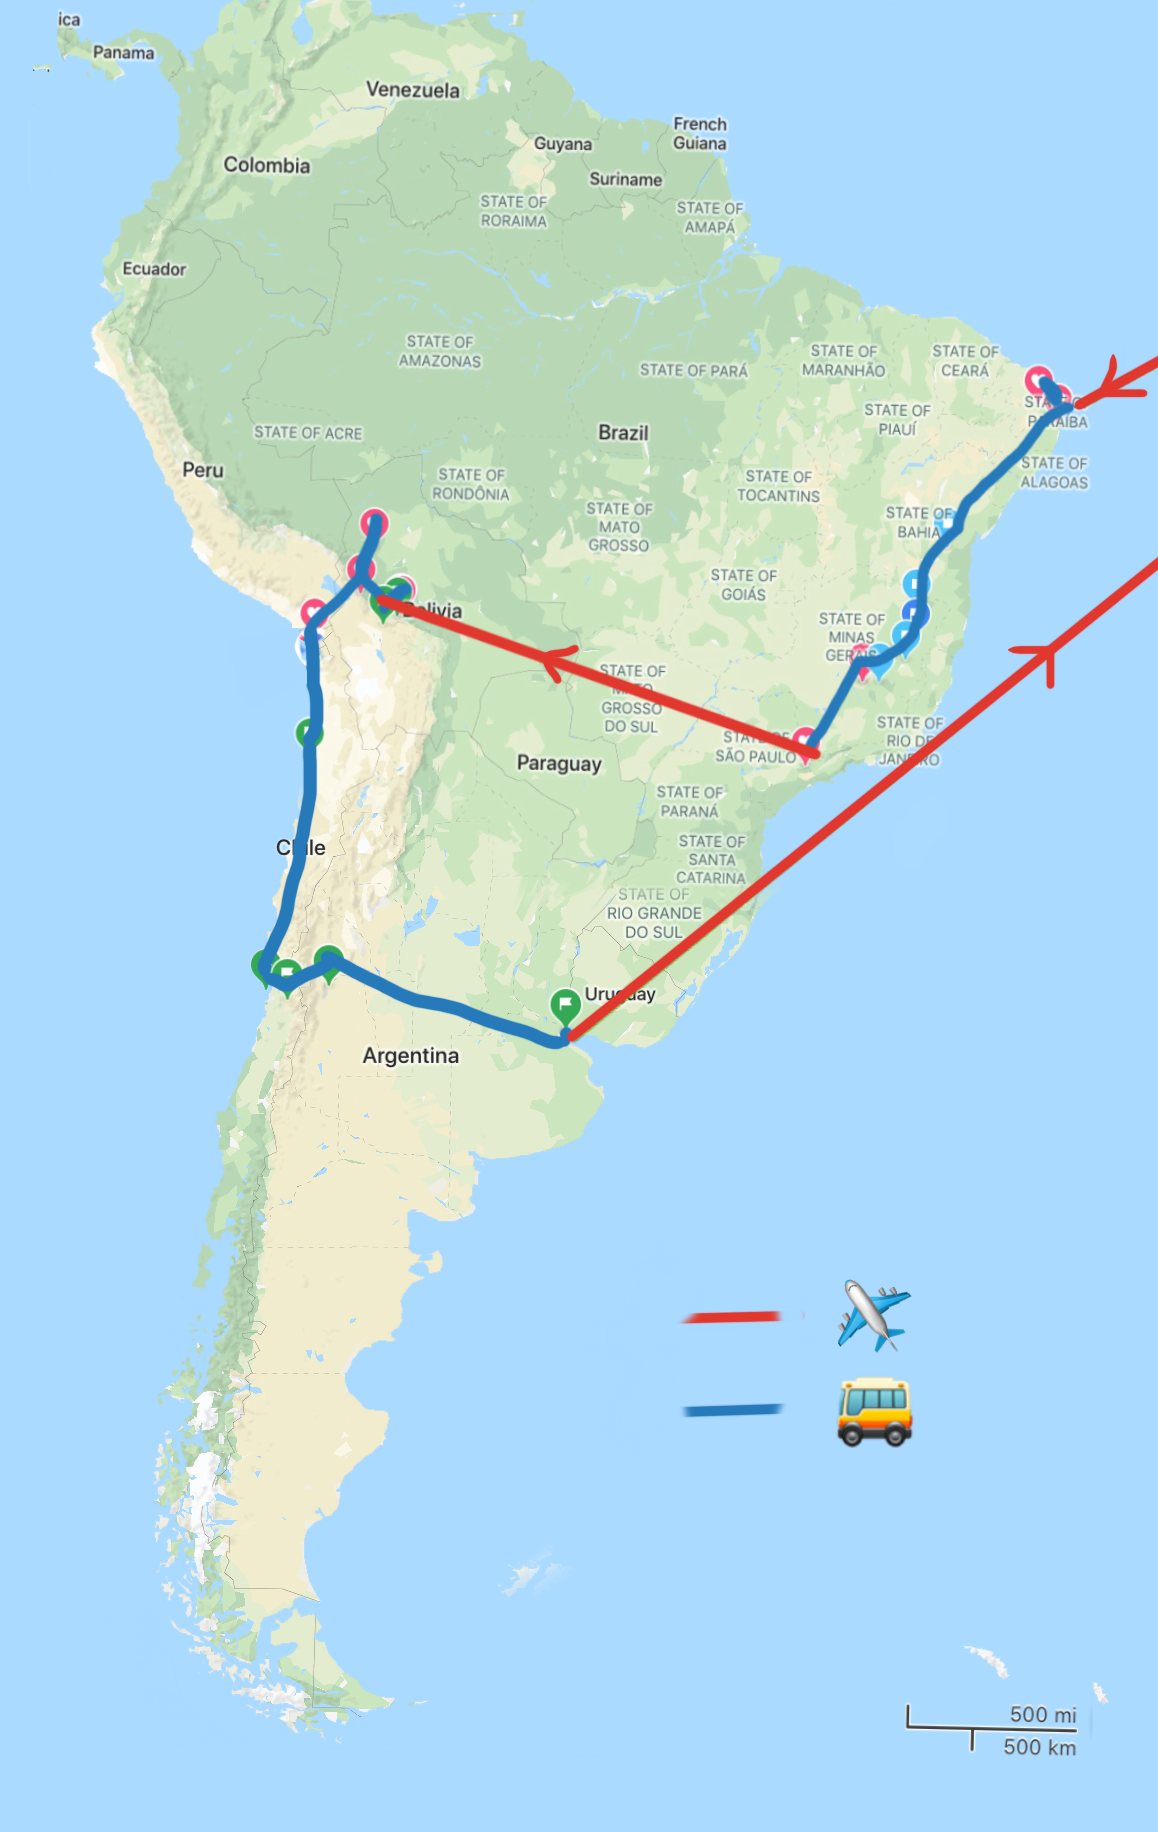
\includegraphics[width=0.9\columnwidth]{trip}
  \caption{Our trip}
\end{figure}

\section{What were the options?}

There were in practice two options to solve the problem:
\begin{itemize}
\item Install a \LaTeX{} system on my iPad.
\item Use an online (cloud-based) \LaTeX{} system.
\end{itemize}

\subsection{\LaTeX{} apps on the iPad}

I found two \LaTeX{} apps on the iOS App Store: Texpad and TeX Writer. Both are offline apps, i.e.\ you don't need an internet connection to compile your \LaTeX{} documents. But, on the other hand, in order to limit the size of the application, they don't have every package from CTAN installed. You can install additional packages, but as iOS is quite a closed operating system, you are dependent on the developers to supply these packages. Of course you have always the option to add the required files to your project directory, but there might be some cases (for example if you need additional fonts) that this is not sufficient.

Also it isn't clear from the documentation of these packages if they can process something like \texttt{.dtx} and \texttt{.ins} files to extract the \texttt{.sty} files and the documentation for the package, which was essential in my case. I got the impression that they were mainly meant for the `normal' user to write articles and reports.

They are also not particularly cheap. At this moment Texpad costs \euro 21.99 and TeX Writer \euro 16.99. If I remember correctly they were a little bit cheaper at the time I was traveling. In itself that is not a very steep price, but I did not expect to use it very often, and just for this single case I thought it was too much. And they don't have a tryout version to see if it really fits you, so if you buy one of these, and you don't like it, you effectively lost your money. And then there is this nagging choice: which of the two is best? All in all, I decided not to go that way.

For the cloud-based systems, I had heard about Overleaf (formerly called WriteLatex) and ShareLaTeX, so I decided to investigate these. It appeared that at that time, these two systems were in a processed of being merged. The result was Overleaf version 2 which had the ShareLaTeX interface, but was still in beta phase. For the simple task that I had, a free account would be sufficient, so I started to try that. However, the merging process introduced some teething troubles. In fact it made editing the files from the iPad browser almost impossible. It wasn't clear if this was a specific problem on the iPad, or that the browser interface in general was not yet mature enough. In effect it wasn't usable at all, because its behaviour was very erratic.

I had also tried to use the Overleaf version 1 interface, but I also could not get that working. I have no idea whether these problems were iPad specific, but anyway I could not use it. By the way, the Overleaf editor is now functioning also on the iPad. However, some functionality is not available without an external keyboard, because they are invoked with control keys. For example the search function is invoked by Control-F on Windows and Linux, and by Command-F on MacOS. On an iPad you can't give these with the virtual keyboard. With an external keyboard it is possible. The current Overleaf editor is reasonable. It has some \TeX-specific functionality. For example, if you type \verb|\begin{enumerate}| the editor adds \verb|\item| and \verb|\end{enumerate}| and positions the cursor after the  \verb|\item| (see figure~\ref{fig:enumerate}).
\begin{figure}[hb]
  \centering
  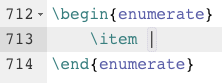
\includegraphics[width=0.9\columnwidth]{enumerate}
  \caption{Editor supplies useful parts}
  \label{fig:enumerate}
\end{figure}

\begin{figure}
  \centering
  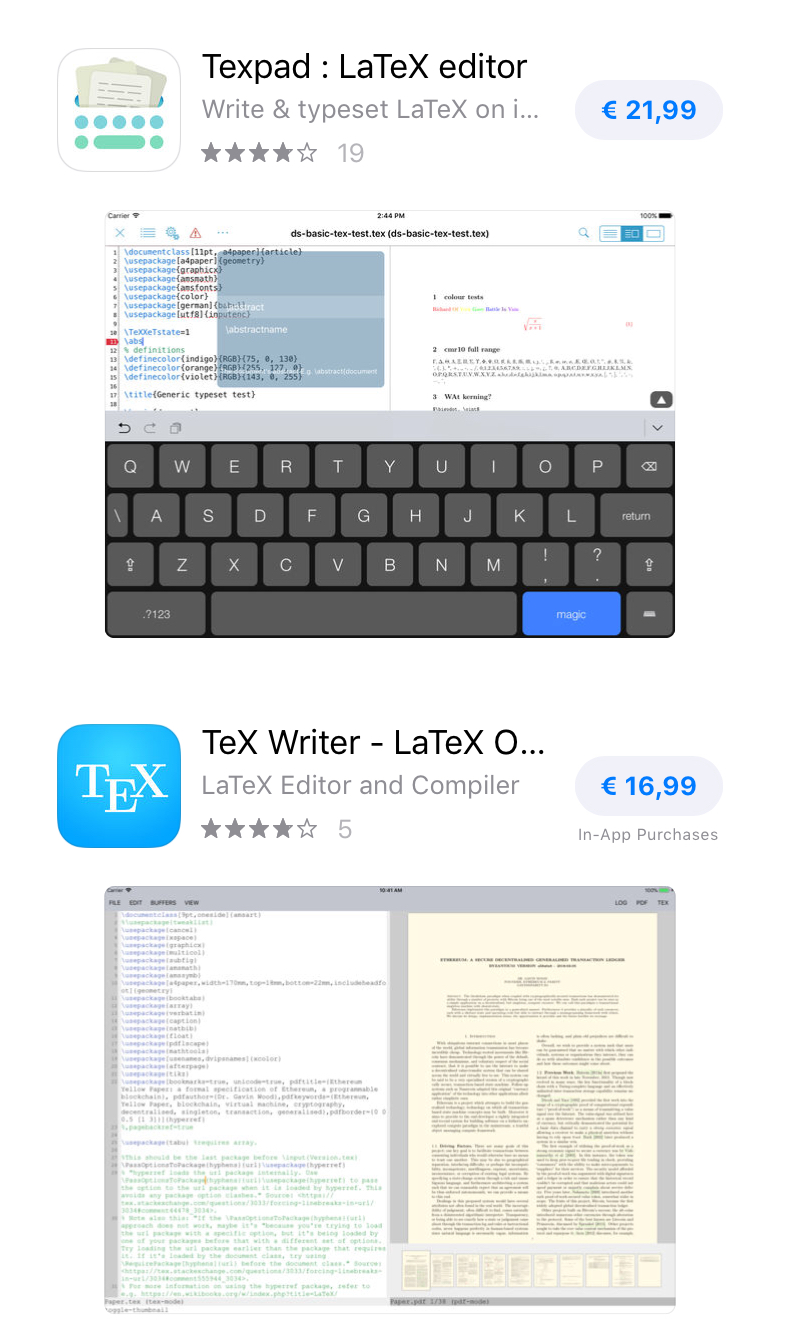
\includegraphics[width=0.9\columnwidth]{ios-apps}
  \caption{Texpad and TeX Writer in the iOS App Store}
\end{figure}

\subsection{Cloud-based \LaTeX{} systems}

\begin{figure*}
  \centering
  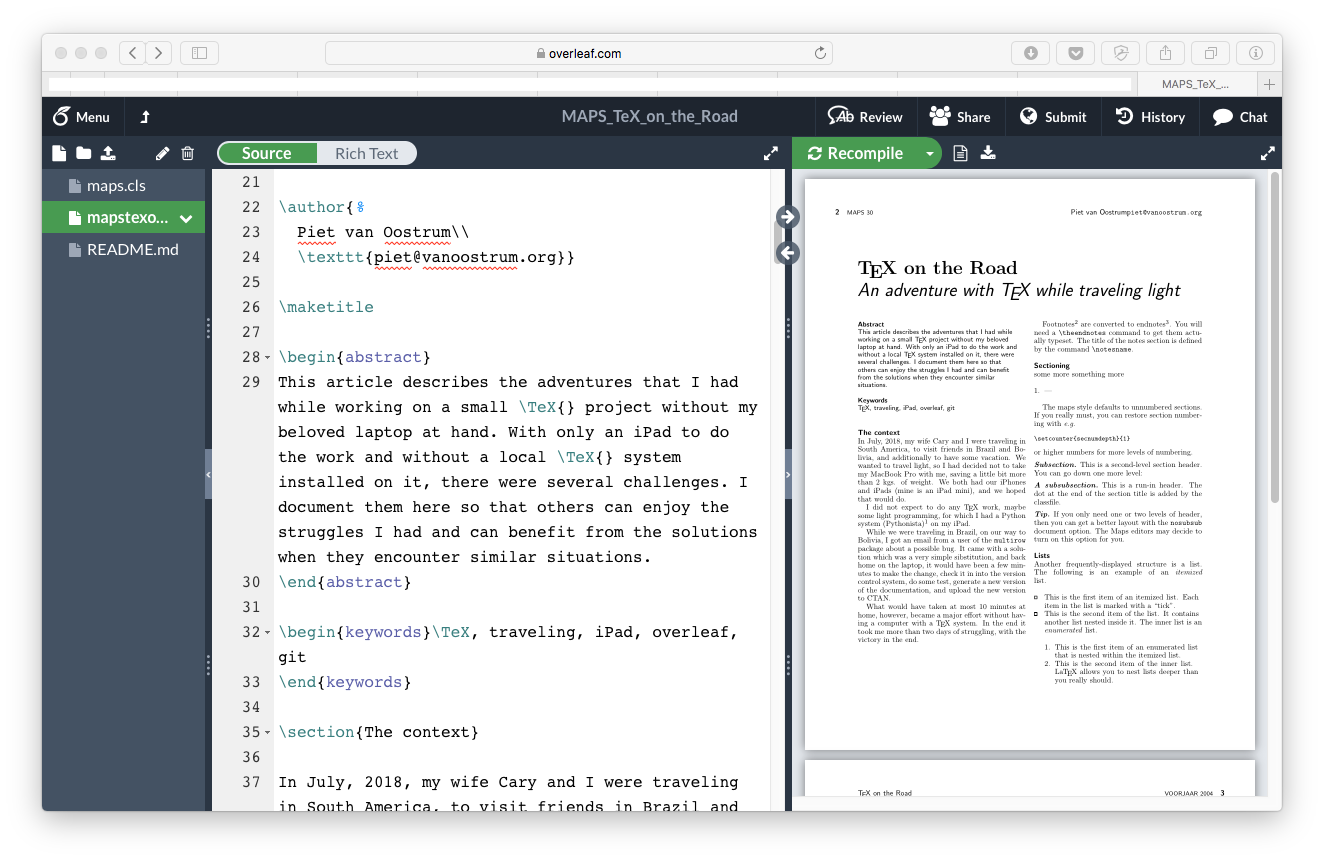
\includegraphics[width=\textwidth]{overleaf}
  \caption{An early version of this article in Overleaf, with some of
    the maps.cls documentation still in place}\label{fig:overleaf}
\end{figure*}

\begin{figure*}
  \centering
  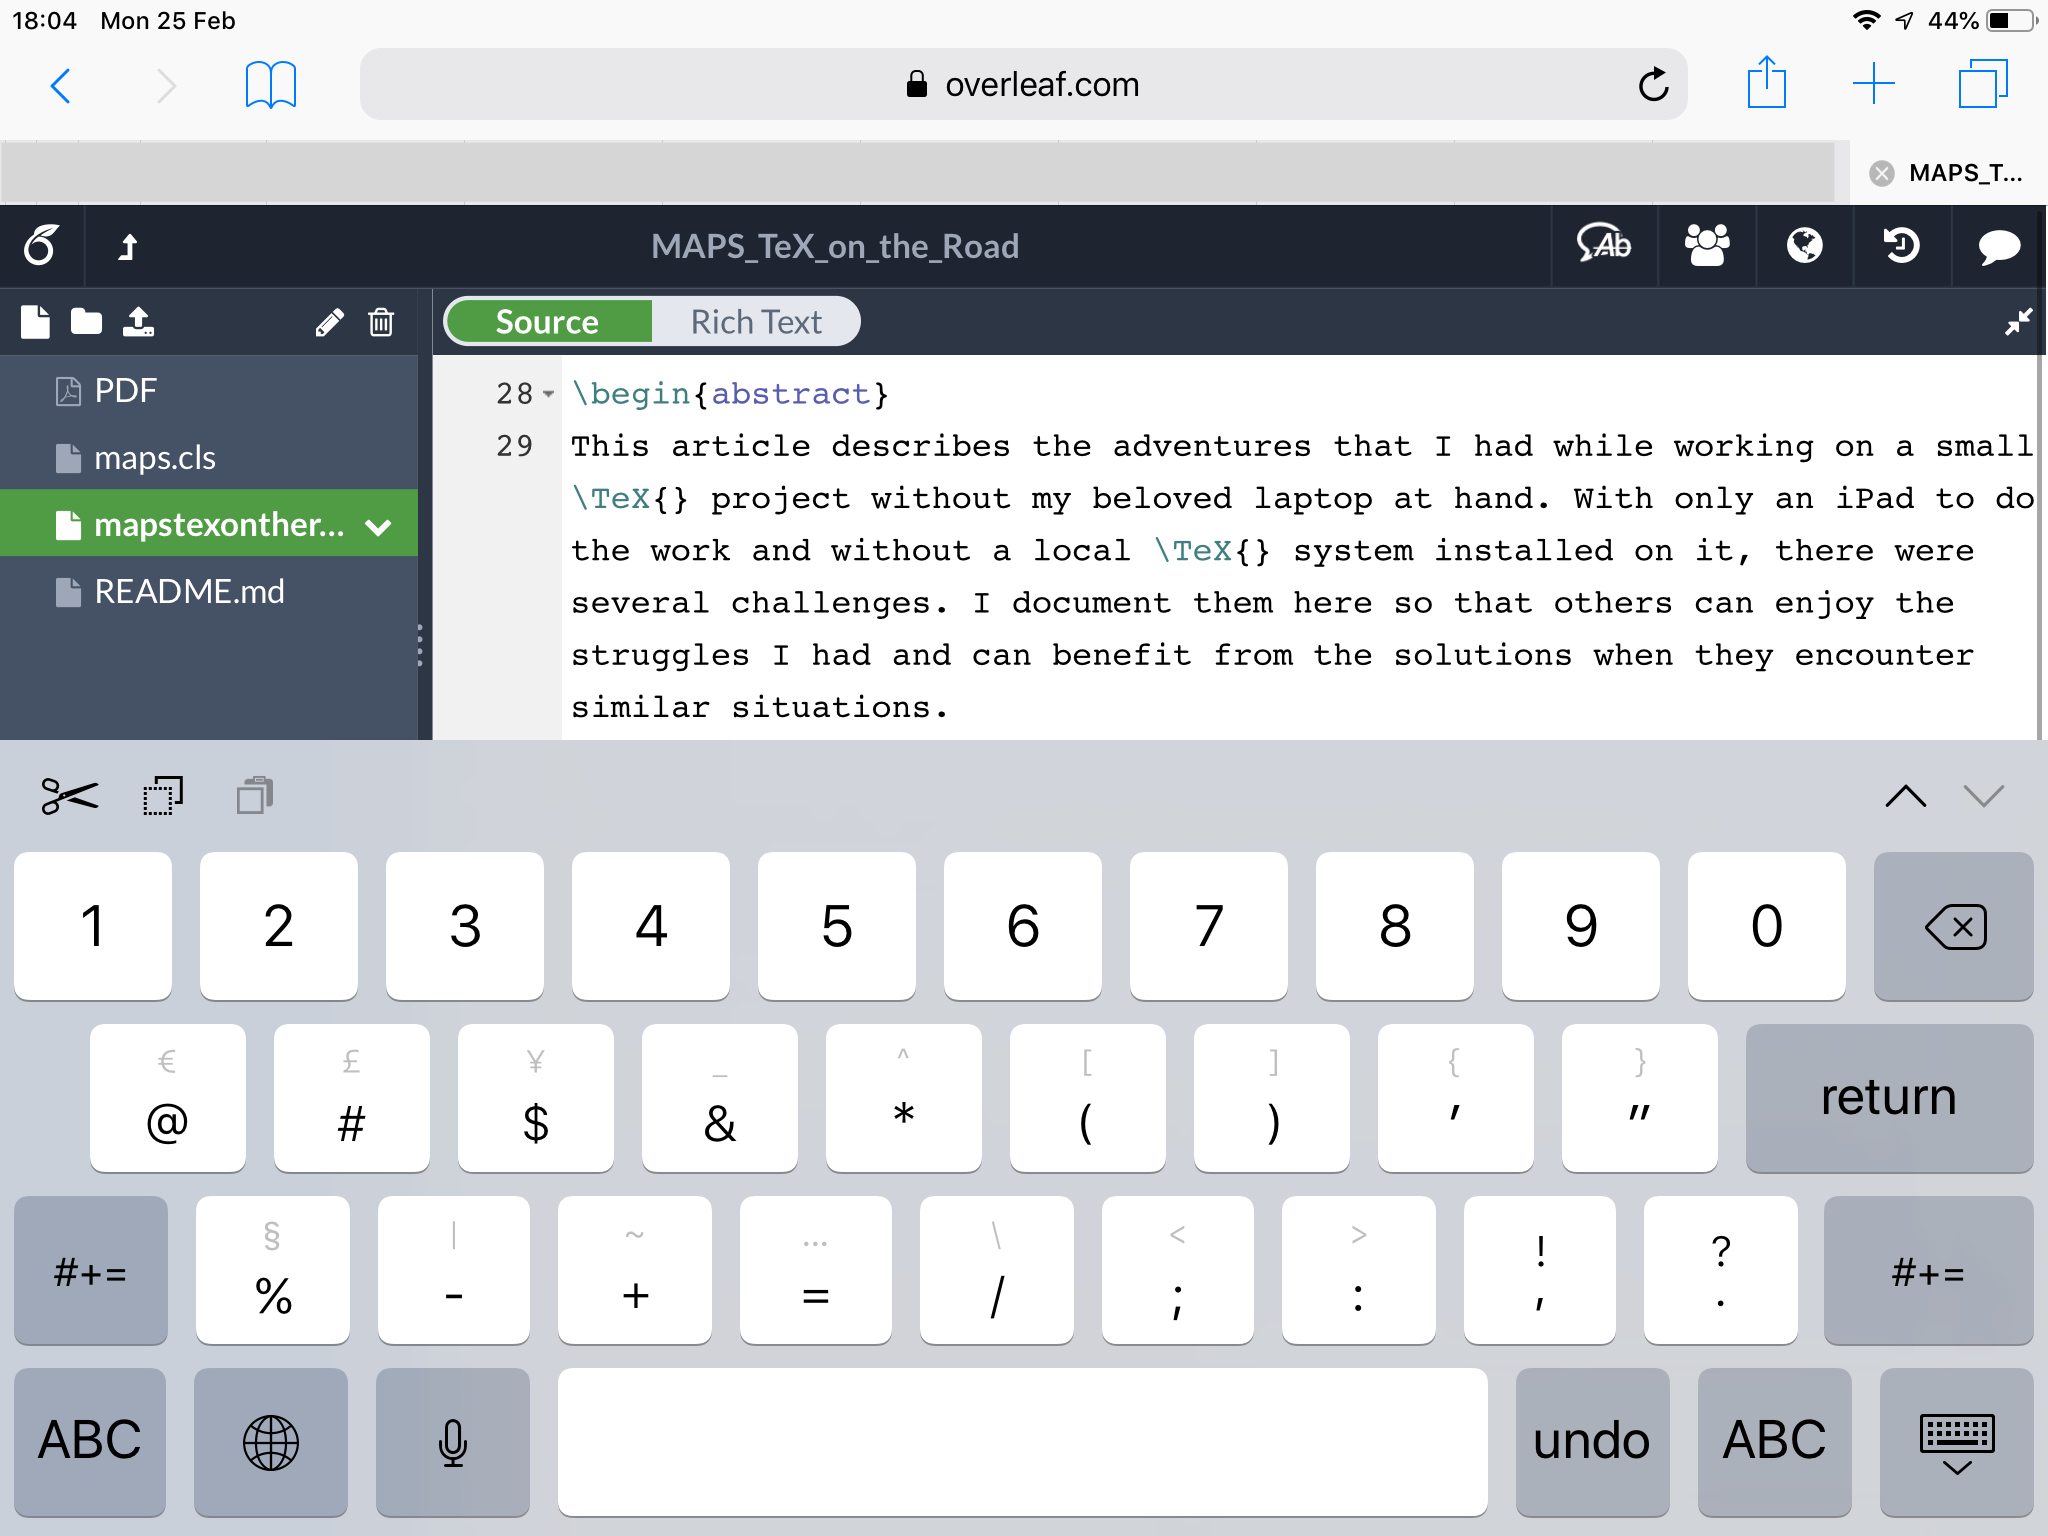
\includegraphics[width=\textwidth]{overleaf-hor}
  \caption{Overleaf screen with virtual keyboard on an iPad}\label{fig:overleaf-hor}
\end{figure*}

\begin{figure*}
  \centering
  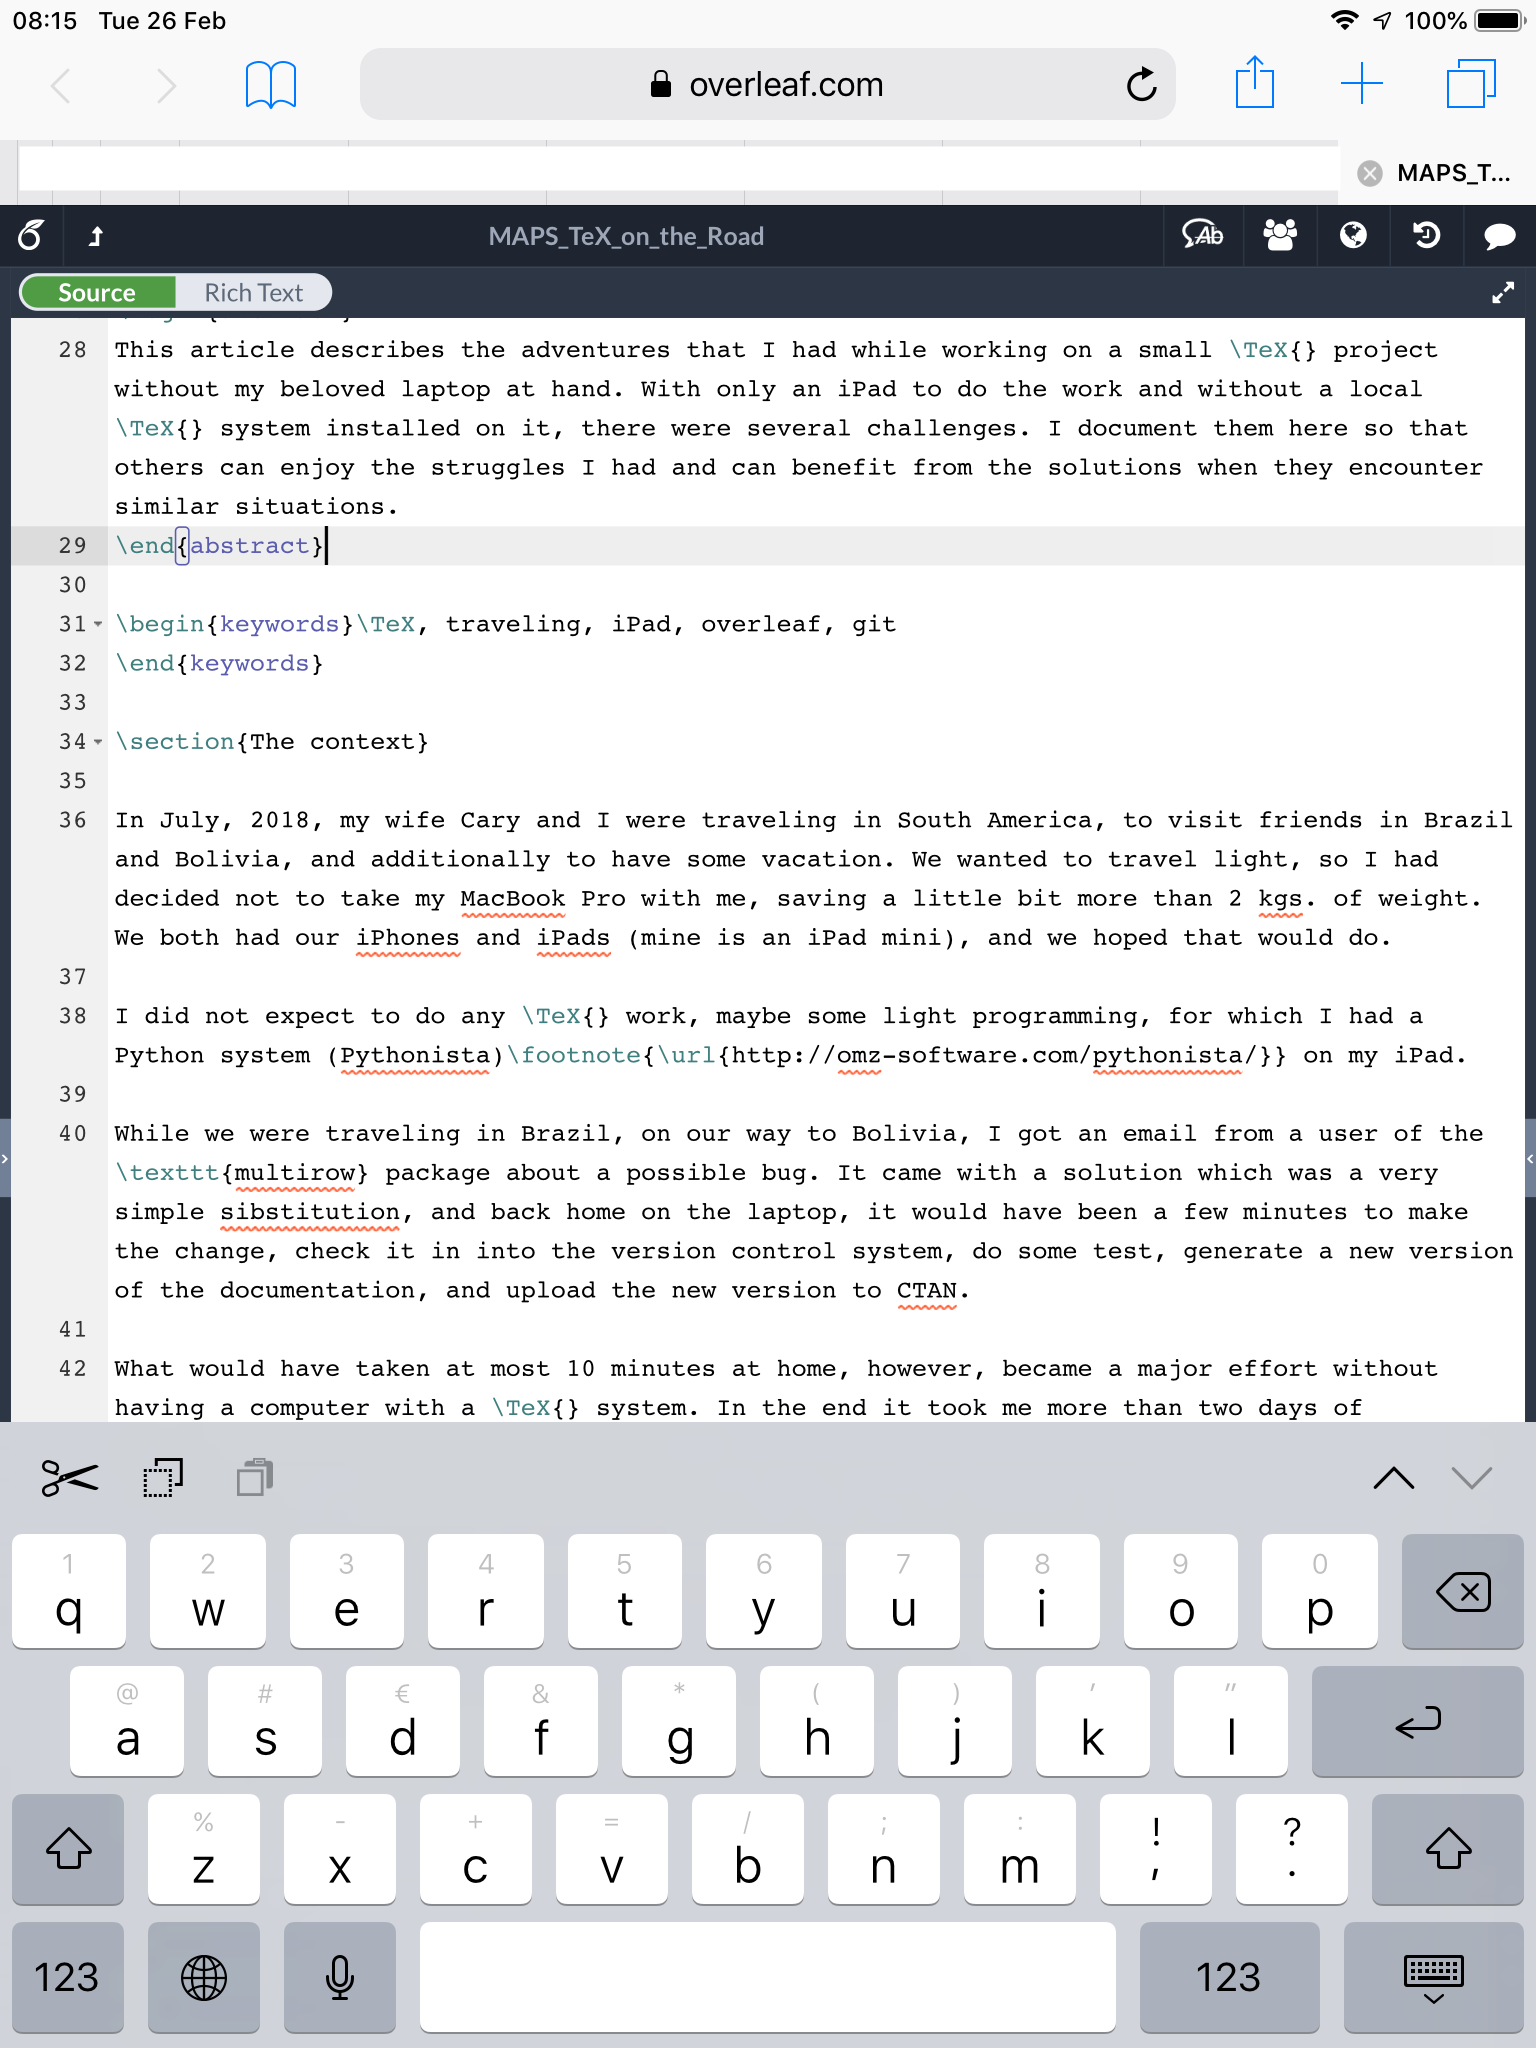
\includegraphics[height=\textwidth]{overleaf-vert}
  \caption{Overleaf screen with virtual keyboard on an iPad in portrait
    mode}
  \label{fig:overleaf-vert}
\end{figure*}

\begin{figure*}
  \centering
  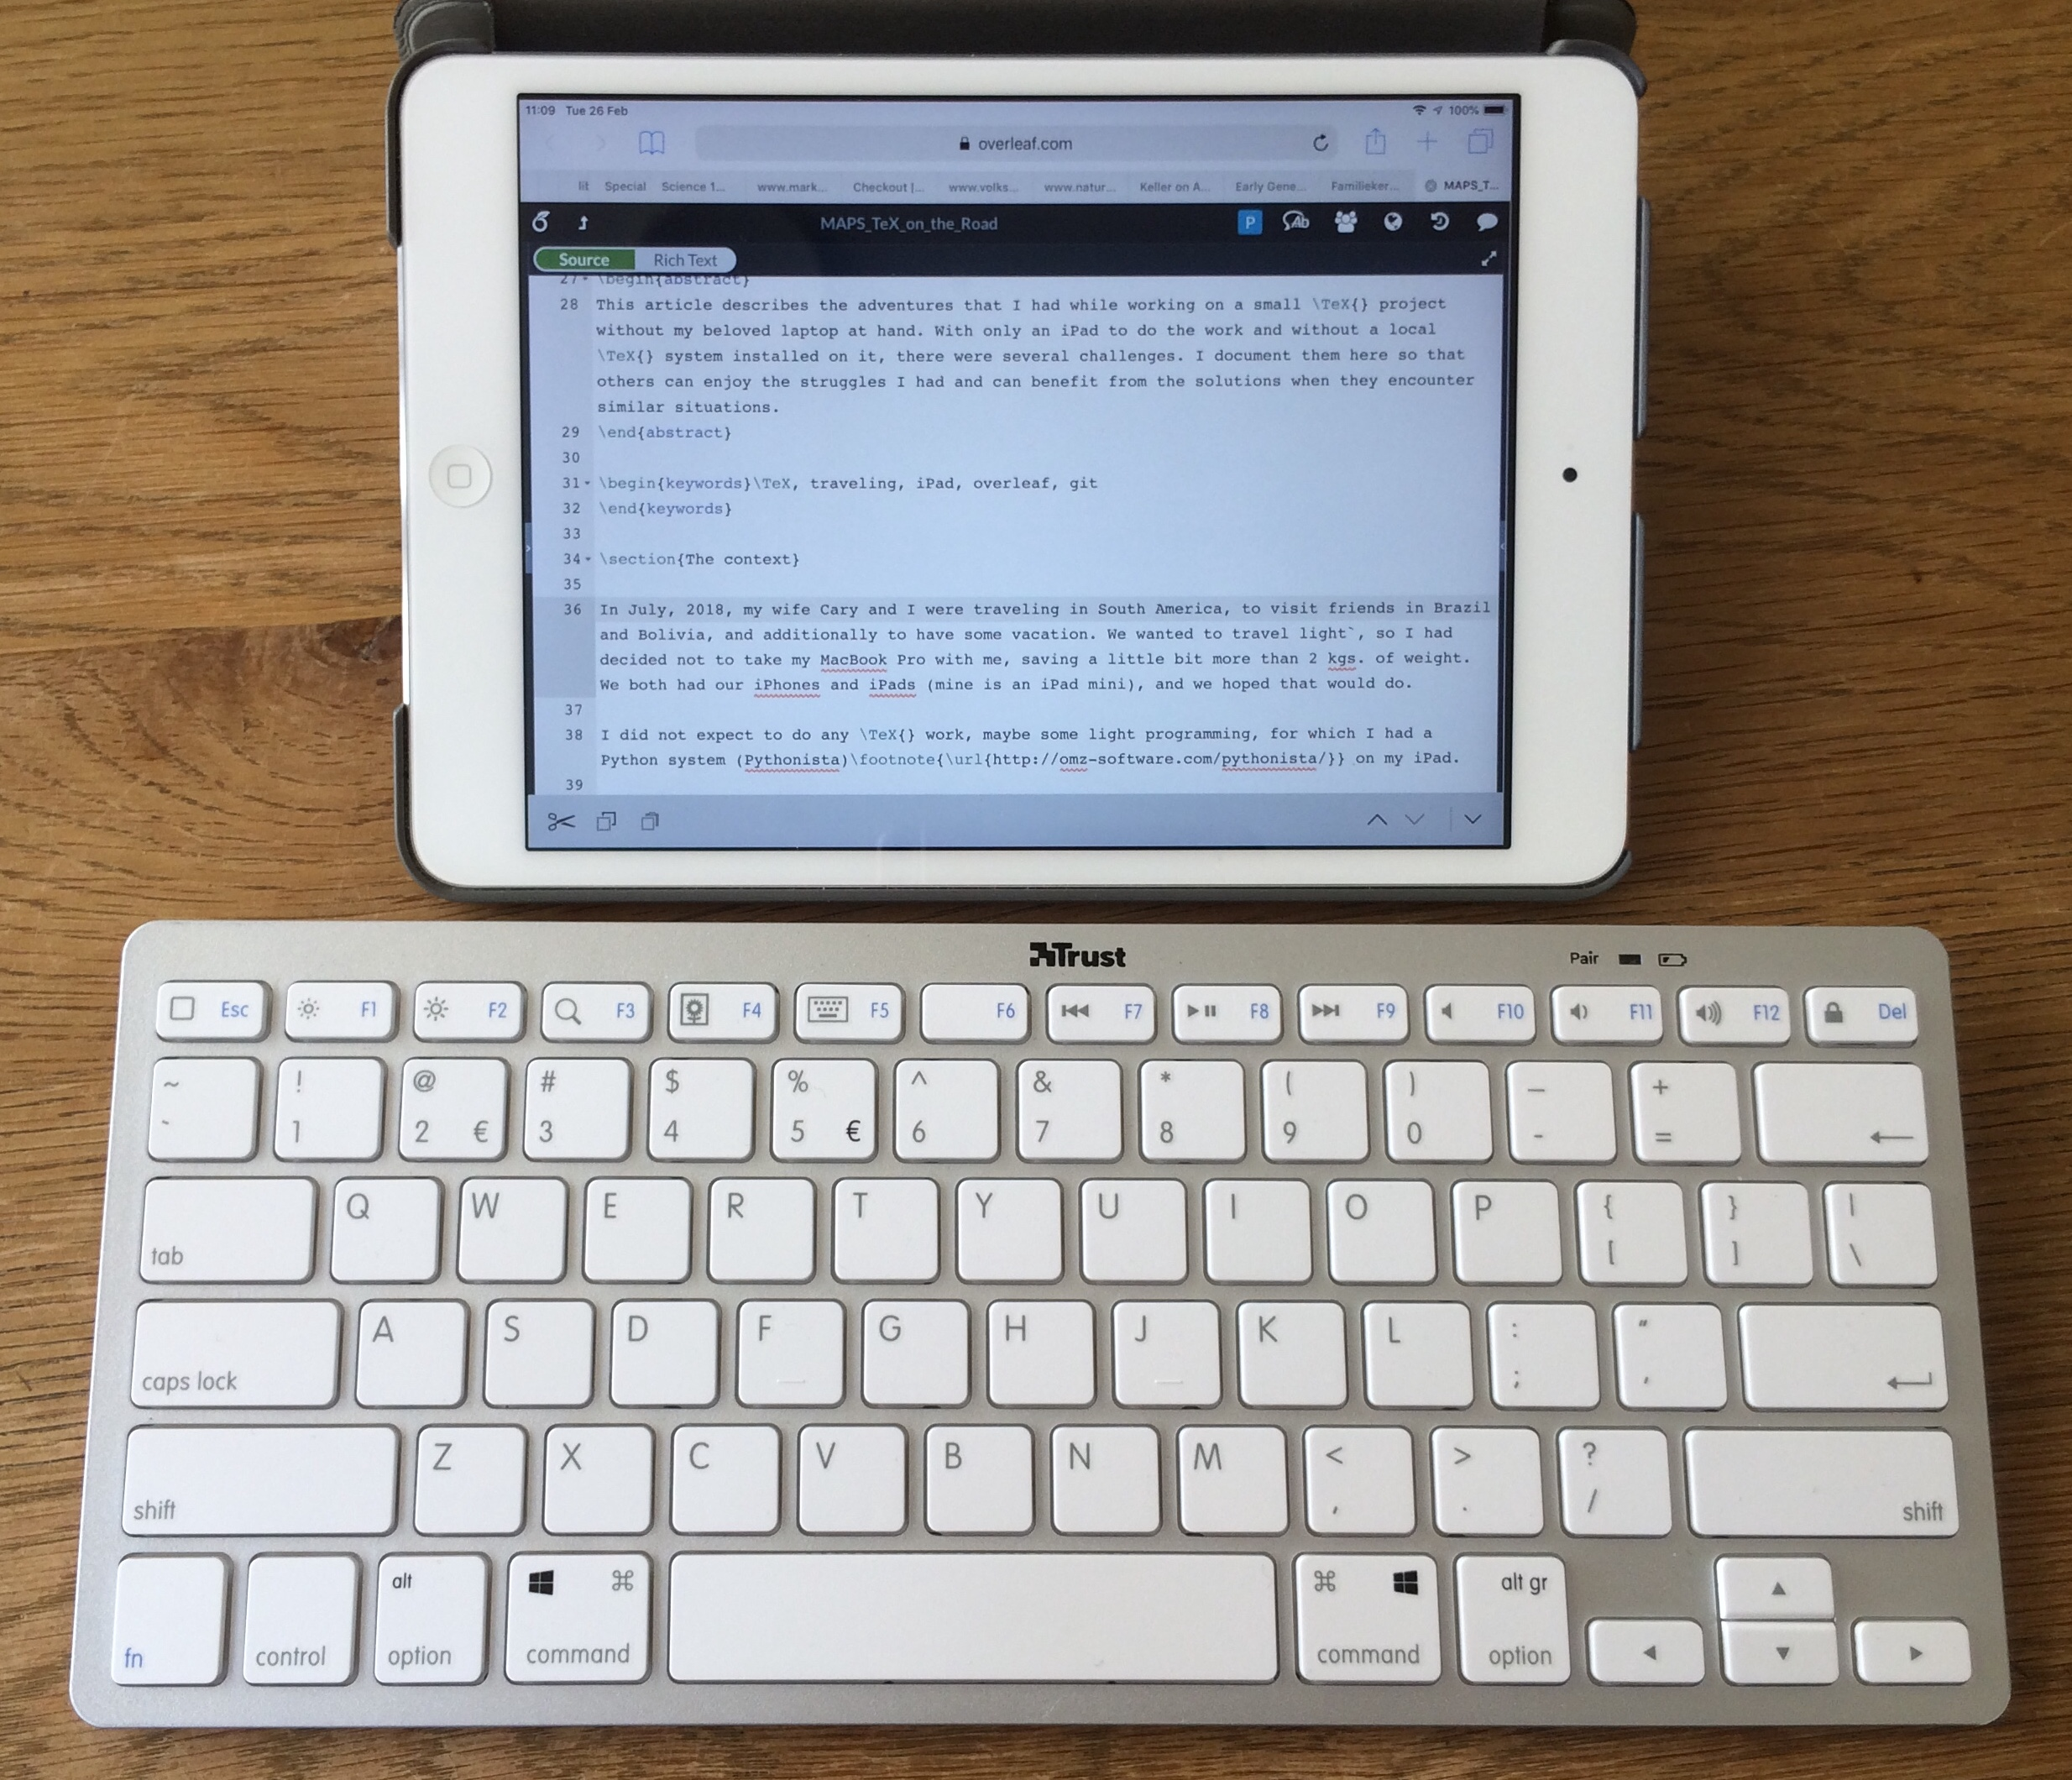
\includegraphics[width=0.9\textwidth]{iPad+keyboard}
  \caption{iPad mini with external keyboard}
  \label{fig:ipad+keyboard}
\end{figure*}

Despite the problems that the editor gave at that time, it seemed to me that this was the best way to go forward. Figure~\ref{fig:overleaf} shows the screen from the current version of Overleaf on my MacBook. The default screen has an edit window with the \LaTeX{} source text and a preview window with the resulting PDF. The preview is not live, you have to hit the Recompile button to update it. There is also a file list on the left and it has the possibility to hide or show each of these parts and to adjust the sizes of each part. Especially on the smaller iPad screen it is advisable to have only the source code part while editing. But even then, the virtual iPad keyboard takes so much space the hardly any source code is visible. See figure~\ref{fig:overleaf-hor}. Also in this case, the file list at the left would make the edit window even smaller, but the file list can be hidden, as shown in the image.

It helps to put the iPad in portrait mode, as shown in figure~\ref{fig:overleaf-vert}. But then the keyboard is rather small. For a setup like this to be workable, it would be better to use an external keyboard. There are several keyboards on the market that can be used. They are generally connected through Bluetooth. They are light-weight and don't take much space, so ideal for traveling light. See figure~\ref{fig:ipad+keyboard}. I did not have one at that moment, however.

\section{Setting up the project}

Setting up the project is easy. You can create a new project in the Overleaf in the Web interface. You can upload each file individually, or a zipfile with everything included. Overleaf will unpack the zipfile in your project.

Immediately, it became apparent that there was a problem with my project. Overleaf wants you to designate one of your files as the main \TeX{} file, which for me would have been \texttt{multirow.dtx}, but it doesn't accept this. It wants to have a \texttt{.tex} file. It does not recognize the \texttt{.dtx} file as a valid \LaTeX{} file. Neither does it want to edit the \texttt{.dtx} file, but as the editor was unusable, this was of a minor concern. I would have to edit the files locally on my iPad anyway.

So I had to give it a \texttt{.tex} file to make it (and myself) happy. I tried two ways
\begin{itemize}
\item Copy \texttt{multirow.dtx} to \texttt{multirow.tex}
\item Make a file \texttt{multirow.tex} that just contains \verb|\include{multirow.dtx}|
\end{itemize}
I had expected that each of these would compile the \texttt{.dtx} file when the Compile button would be pressed. However, it didn't. It took some time to find out why. My \texttt{multirow.dtx} contains a line
\begin{verbatim}
\DocInput{\jobname.dtx}
\end{verbatim}
which is quite usual. After some searching I found out that \verb|\jobname| wasn't \texttt{multirow} as was to be expected, but \texttt{output}. It appears that Overleaf runs the job in a kind of \textit{sandbox} with the name of the main file \texttt{output}.

After some googling I found that Overleaf uses \texttt{latexmkrc} to process the job. It provides a standard, but invisible, \texttt{latexmkrc} file that controls the compilation process. However, you can also supply your \texttt{latexmkrc} file. This file is described in section~\ref{sec:latexmk}.

So the challenge was now to upload a correct \texttt{latexmkrc} file, and to update the \texttt{multirow.dtx} file. This could be done by uploading these files after each modification, but this might be an error-prone process, and you don't have a record of what has been done. Enter version management.

\section{Distributed version management}

In any project where you have to make changes more or less regularly, it is important to keep track of what you have done. Also, in general it is useful to have access to previous versions of your project, for example if you want to go back to a previous situation. Some people do this by making copies of their files at regular moments. Sometimes they put the date and the time in the file names, to keep a kind of history. But this becomes soon unwieldy. This is the problem that version management system (also called version control systems) offer a solution for. Each serious developer, whether it is of software or of texts, should consider using a version management system.

For those readers that are unfamiliar with version management, here follows a brief description.
You have a \textit{working copy}, which is the collection of files that you work upon in your project. This is just like when you do not use version management. Additionally you have a \textit{repository}, which is a kind of database containing the history of your project. It will contain the state of your \textit{working copy} at certain moments in the past, together with information about who made the changes, and a description of what has changed.

If, at a certain moment, you have a state of your project that you want to keep, you \texttt{commit}, which means a copy is made to the \texttt{repository}, together with a description that you enter. You usually have a separate repository for each project. The repository can be on your local computer, or on a server. In the latter case it is possible that different people working on the same project use the same repository. They would then each have their own \texttt{working copy}. As they are working independently, these could be different. A version management system usually has provisions to resolve conflicting working copies.

There are several version management systems available. One older, well-known system is \textit{subversion} (SVN\footnote{\url{http://subversion.apache.org}}). It usually has the repositories at a central server, but you can also have the repository on your local computer, if you are working alone. As SVN has only one repository per project it is called a centralized version management system.

Centralized version management systems have some big disadvantages for cooperation in teams:
\begin{itemize}
\item If you work together the repository must be on a central server, which means you cannot use it when you are off-line.
\item If you want to keep your changes registered often in the repository, then this can be confusing for the other team members. On the other hand, if you want to keep the repository relatively clean, that is, only commit major updates, then you lose the possibility to keep your own history detailed.
\end{itemize}
One solution would be to have both a central repository for the team, and your local repository for your own work, but then synchronizing these repositories could become tedious. However, this is where \textit{distributed version management systems} have their strength.




\newpage \null \newpage

\section{Lists}

Another frequently-displayed structure is a list.
The following is an example of an \emph{itemized}
list.
\begin{itemize}
  \item This is the first item of an itemized list.
    Each item in the list is marked with a ``tick''.
  \item This is the second item of the list.  It
    contains another list nested inside it.  The inner
    list is an \emph{enumerated} list.
    \begin{enumerate}
      \item This is the first item of an enumerated
        list that is nested within the itemized list.

      \item This is the second item of the inner list.
        \LaTeX\ allows you to nest lists deeper than
          you really should.
    \end{enumerate}
    This is the rest of the second item of the outer
    list.  It is no more interesting than any other
    part of the item.
  \item This is the third item of the list.
\end{itemize}
In a two-column layout, protracted indenting doesn't look very
good. Therefore, the Maps classfile provides \texttt{itemouter}- and
\texttt{enumouter} environments:
\begin{itemouter}
\item This is the first item of a non-indented itemized list,
  produced with the \texttt{itemouter} environment.
\item This is the second item.
\end{itemouter}
Now an enumerated version:
\begin{enumouter}
\item This is the first item of a non-indented enumerated list,
  produced with the \texttt{enumouter} environment.
\item This is the second item.
\end{enumouter}
And a version for descriptions:
\begin{descript}
\item[cow] A milk-producing animal that grazes grass and has
multiple stomachs
\item[kangoroo] An Australian hopping animal
\end{descript}

\section{Tabulars}

The Maps classfile adds some vertical space around horizontal rules in
tables. This makes vertical rules look funny, but most of the time you
are better off without vertical rules anyway; see table~\ref{tabulars}.
If you really insist on vertical rules, use the \texttt{deftables}
document option.

\begin{table}[ht]

\begin{tabular}{|l|l|}
\hline
var & value\\
\hline
$Q_{s,\max}$ & 0.18\\
$K_{s}$      & 1.0\\
$Y_{x/s}$    & 0.5\\
$Y_{p/s}$    & 0.854\\
$Q_{p,\max}$ & 0.0045\\
$\mu_{\rm crit}$  & 0.01\\
$k_{h}$       & 0.002\\
$m_{s}$       & 0.025\\
\hline
\end{tabular}\hspace{2pc}
\begin{tabular}{@{}ll@{}}
\hline
var & value\\
\hline
$Q_{s,\max}$   & 0.18\\
$K_{s}$        & 1.0\\
$Y_{x/s}$      & 0.5\\
$Y_{p/s}$      & 0.854\\
$Q_{p,\max}$   & 0.0045\\
$\mu_{\rm crit}$ & 0.01\\
$k_{h}$        & 0.002\\
$m_{s}$        & 0.025\\
\hline
\end{tabular}
\caption{Tabulars with and without vertical rules}\label{tabulars}
\end{table}

\section{Wide typesetting in single-column layout}

For both single-column layouts, there are environments \texttt{fullwidth} and
\texttt{verboutdent} which typeset their content across the full page,
including most of the wide margin.

\begin{fullwidth}
x x x x x x x x x x x x x x x x x x x x x
x x x x x x x x x x x x x x x x x x x x x
x x x x x x x x x x x x x x x x x x x x x
x x x x x x x x x x x x x x x x x x x x x
\end{fullwidth}

\begin{verboutdent}
{}\/$xxxxxxxxxxxxxxxxxxxxxxxxxxxxxxxxxxxx
\end{verboutdent}
The implementation of \texttt{fullwidth} is rather simplistic and
may easily break, in which case more sophisticated hackery will be
needed.

\section{Fonts}

At production time, Computer Modern will be replaced with Bitstream
Charter, scaled to 95\%, and Latin Modern. For math, the eulervm
package will be used. You can safely ignore warnings about size
substitutions.

\section{Assembling your submission}

Please check whether all non-standard stylefiles and packages and all
non-standard fonts are included. We do have a current \TeX{} Live but,
although we do have access to CTAN, finding the right package by
name can occasionally be a challenge.

Avoid jpeg compression for screenshots. Conversion to pdf may
sometimes result in jpeg compression as well. Use \emph{e.g.} png
format instead.

Finally, a pdf of your article is appreciated. This way, we can
check more reliably whether your article compiles
correctly on our own systems.

\section{References}

If you have references, use whatever suits you. A few sample references:
see \cite{knuth}, \cite{mapsclass} or \cite{lamport}.

\theendnotes

%\bibliographystyle{apalike}
%\bibliography{maps}

\begin{thebibliography}{}

\bibitem[Knuth, 1986]{knuth}
Knuth, D.~E. (1986).
\newblock {\em The {\TeX{}}book}.
\newblock Addison-Wesley Publishing Company.

\bibitem[Kroonenberg, 2004]{mapsclass}
Kroonenberg, S. (2004).
\newblock The maps style.
\newblock {\em Maps}, 30.

\bibitem[Lamport, 1994]{lamport}
Lamport, L. (1994).
\newblock {\em {\LaTeX} a Document Preparation System}.
\newblock Addison-Wesley Publishing Company, 2nd edition.

\end{thebibliography}

\end{document}

%%%%%%%%%%%%%%%%%%%%%%%%%%%%%%%
% the bibtex file:

@BOOK{knuth,
author = "Donald E. Knuth",
title = "The {\TeX{}}book",
publisher = "Addison-Wesley Publishing Company",
year = 1986,
}

@BOOK{lamport,
author = "Leslie Lamport",
title = "{\LaTeX} a Document Preparation System",
publisher = "Addison-Wesley Publishing Company",
edition = "2nd",
year = 1994,
}

@ARTICLE{mapsclass,
author = "Siep Kroonenberg",
title = "The Maps style",
journal = "Maps",
volume = "30",
year = "2004"
}
